\section{Introduction}

\begin{frame}{Introduction}
    What problem did we try to solve?
\end{frame}

\begin{frame}{Introduction}
    \begin{center}
        \begin{figure}[H]
            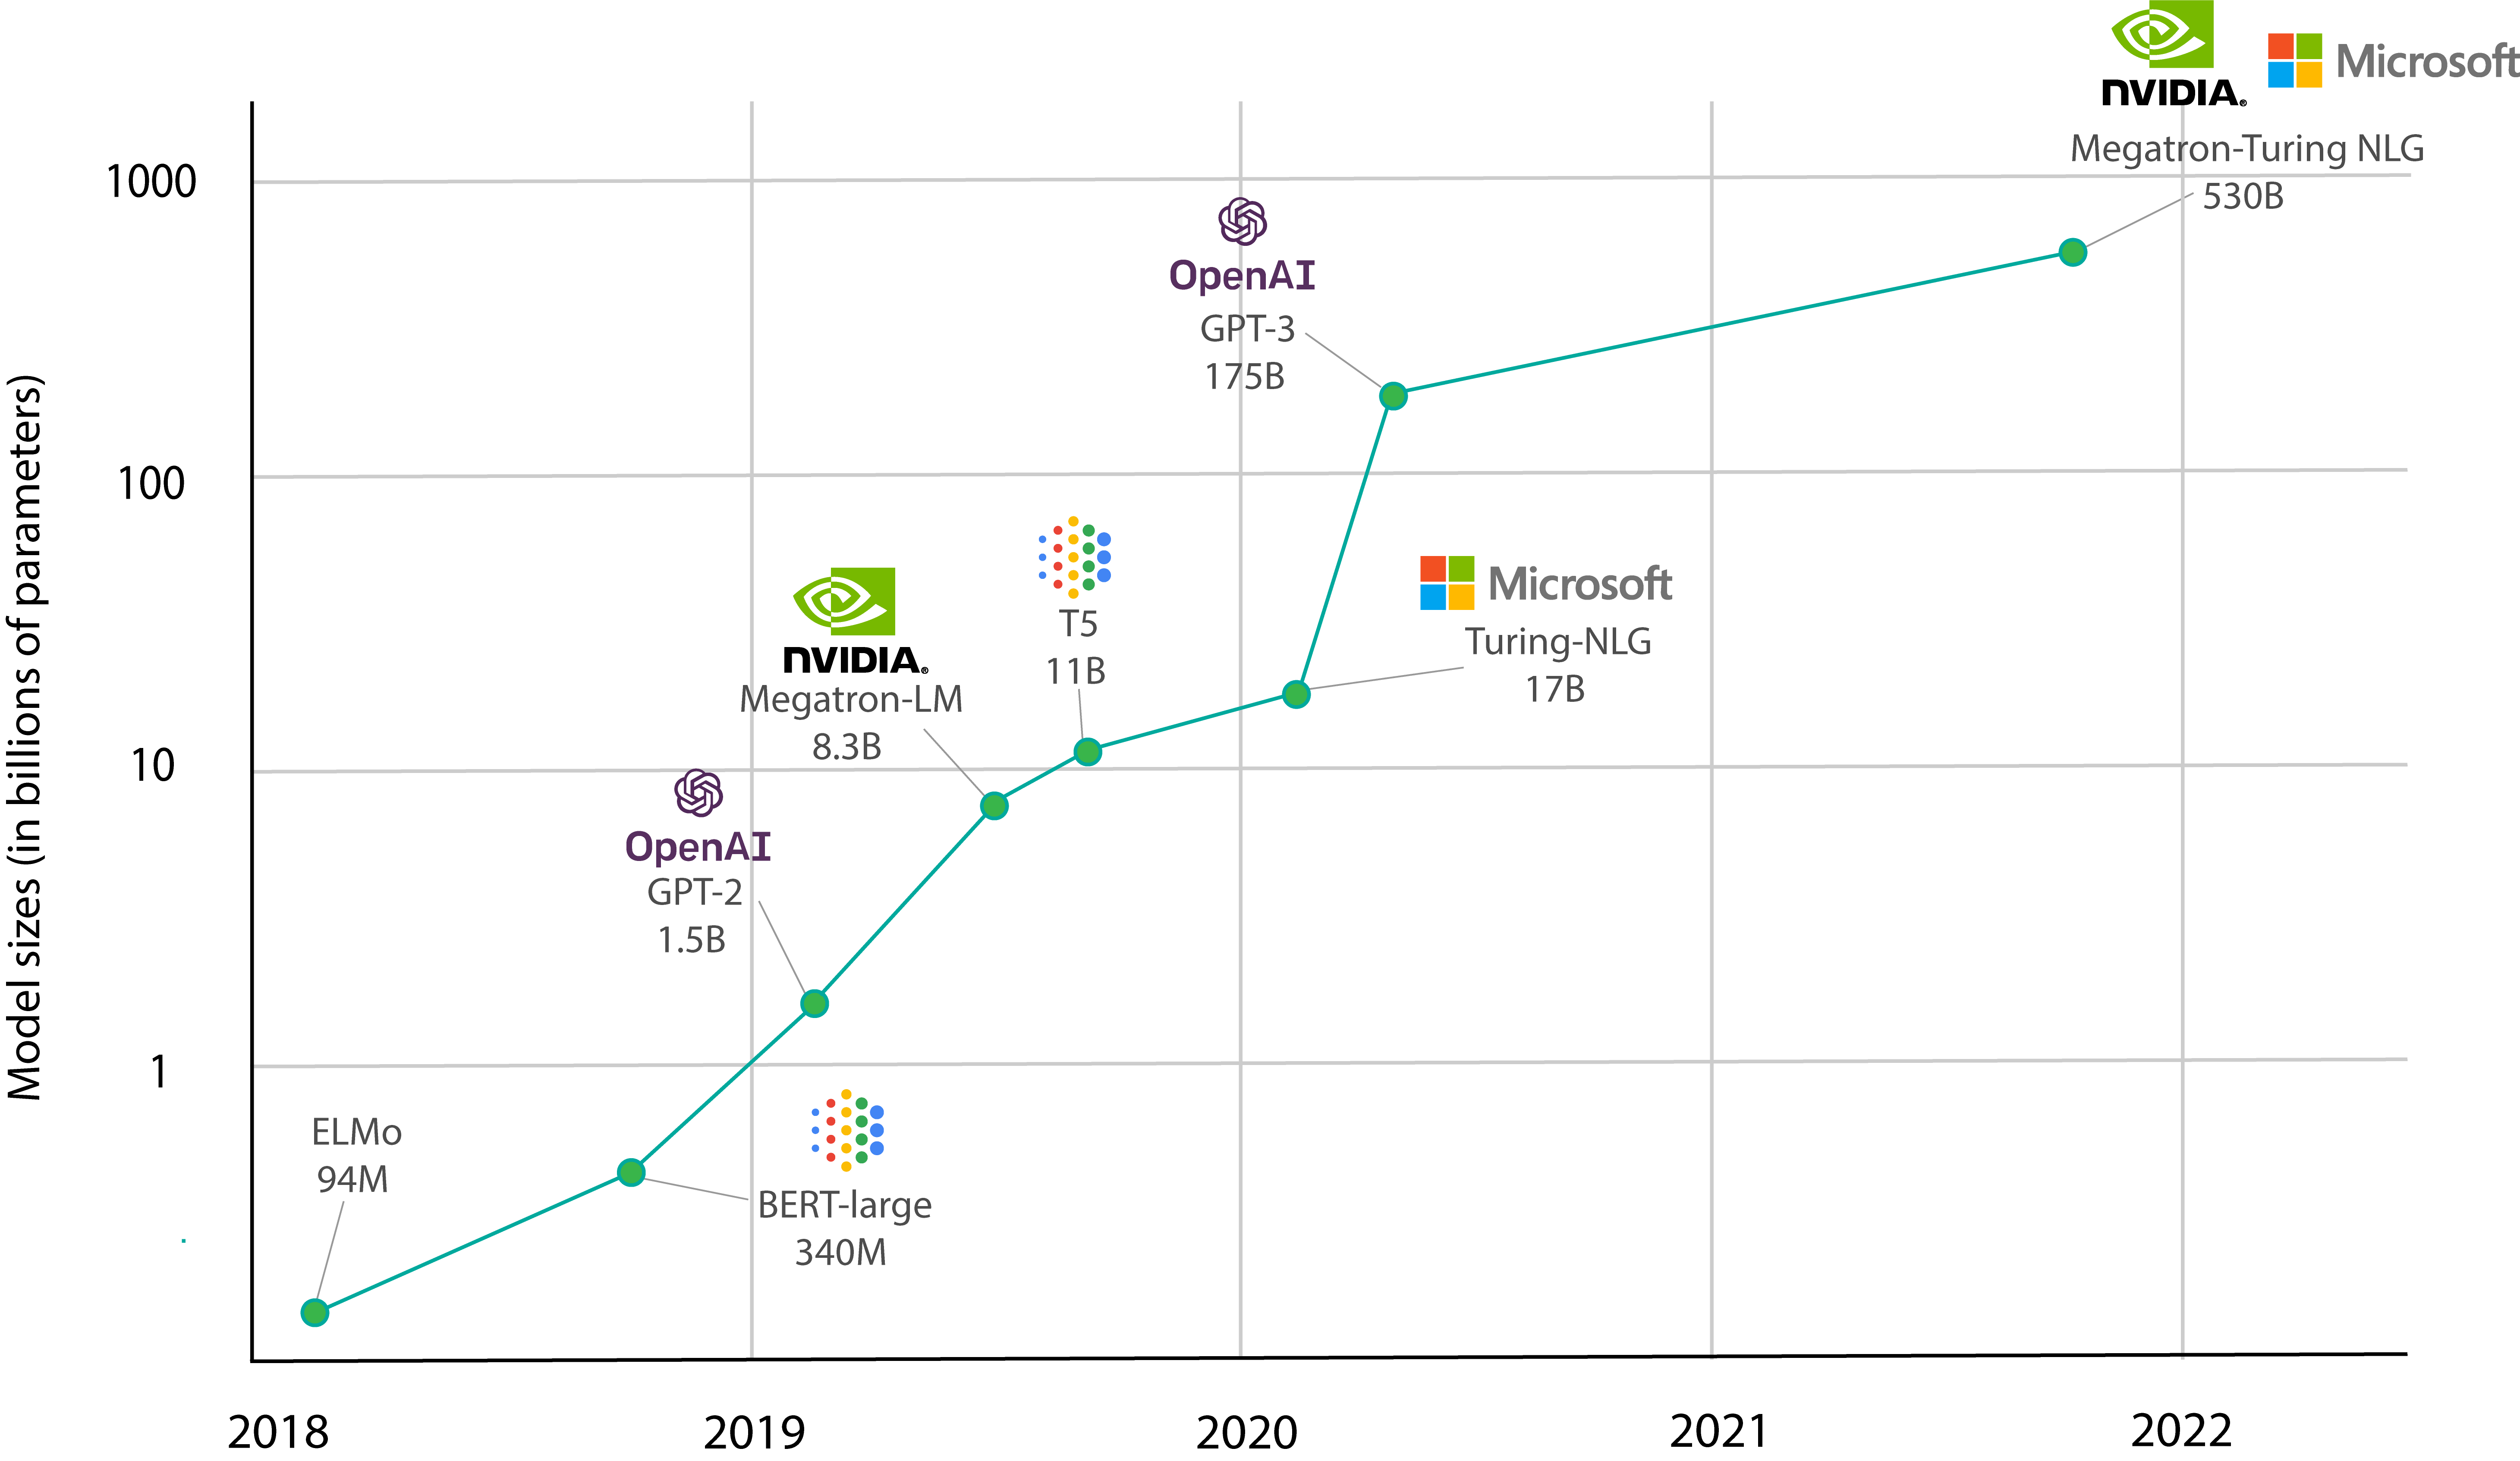
\includegraphics[scale=.4]{figures/introduction/big_language_models.png}
        \end{figure}
    \end{center}
\end{frame}

\begin{frame}{Introduction}
    Key challenges for large-scale model training:

    \begin{center}
        \begin{itemize}
            \bitem High memory requirements (cost intensive)
            \bitem Long training time  (cost intensive)
            \bitem Scalability in general (Linear scalability?)
        \end{itemize}
    \end{center}
\end{frame}

\begin{frame}{Introduction}
    \begin{center}
        \begin{figure}[H]
            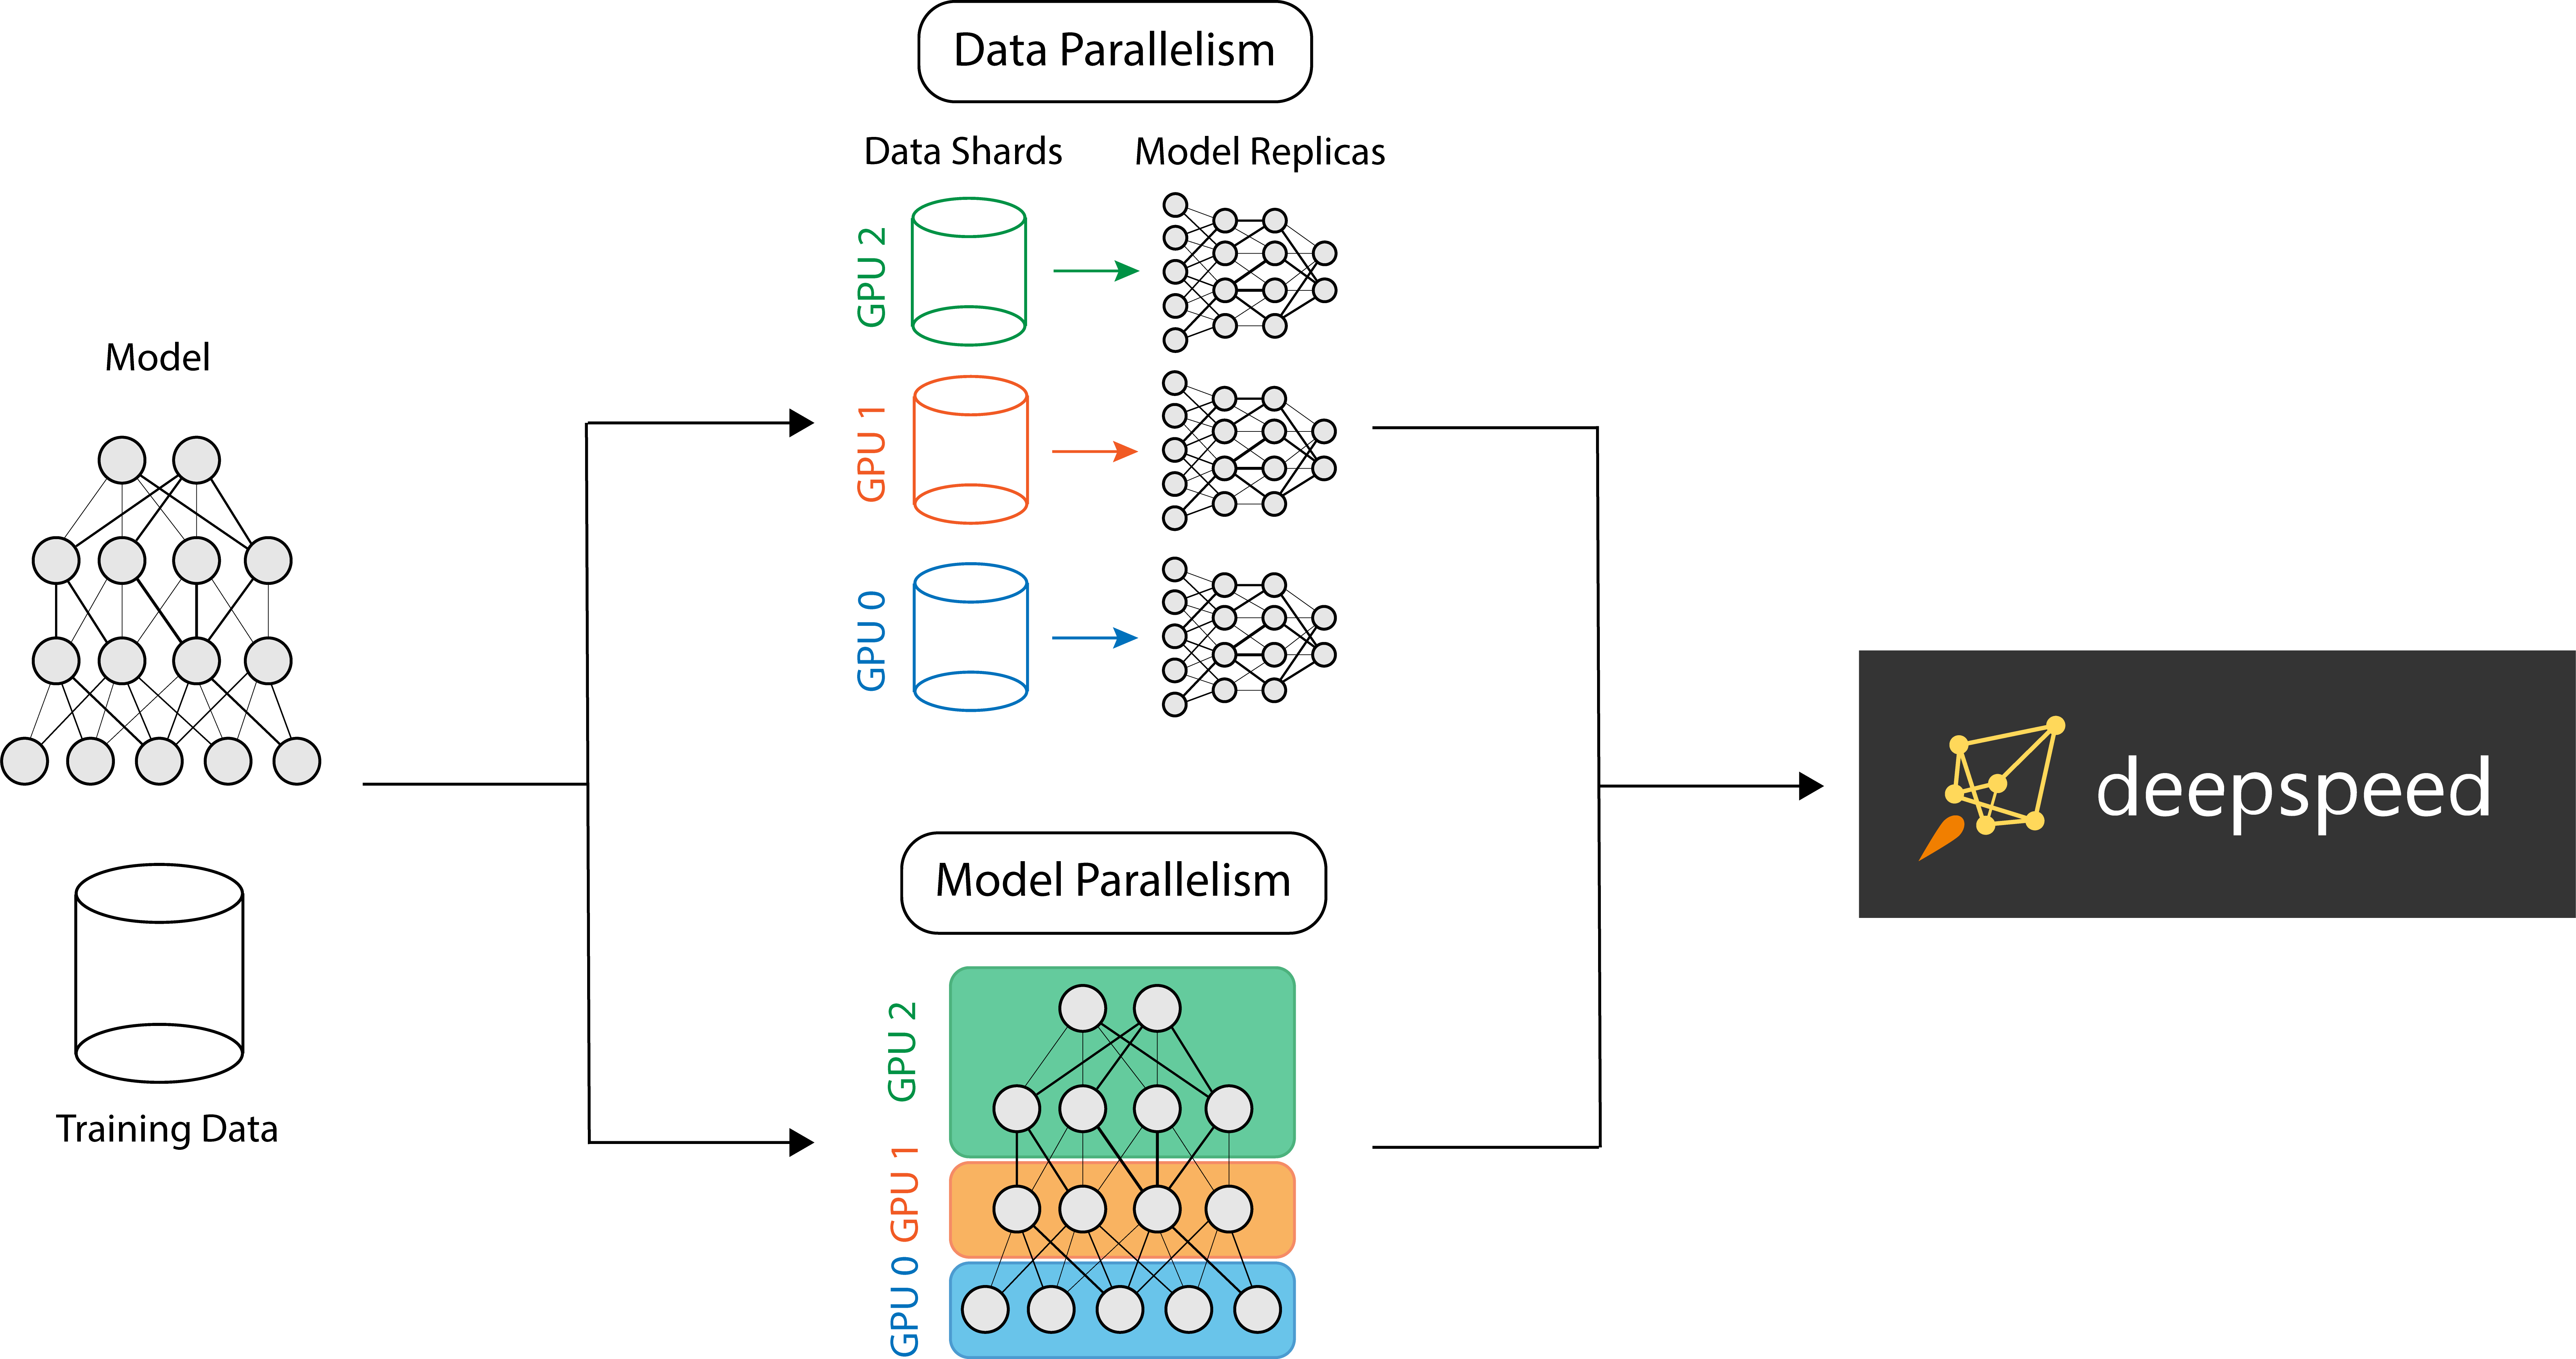
\includegraphics[scale=.35]{figures/introduction/dp-mp-deepspeed.png}
        \end{figure}
    \end{center}
\end{frame}

\begin{frame}{Introduction}
    \begin{columns}
        \begin{column}{{0.5\textwidth}}
            \begin{itemize}
                \bitem Other model architecture than Transformers also profit 
                from scaling to billions of parameters
                \bitem Graph Neural Networks (GNN) have shown promising results 
                in molecular simulations
                \bitem What happens if we apply scaling methods from DeepSpeed 
                to GNNs? 
            \end{itemize}
        \end{column}

        \begin{column}{{0.5\textwidth}}
            \begin{center}
                \begin{figure}[H]
                    \centering
                    \captionsetup{justification=centering}
                    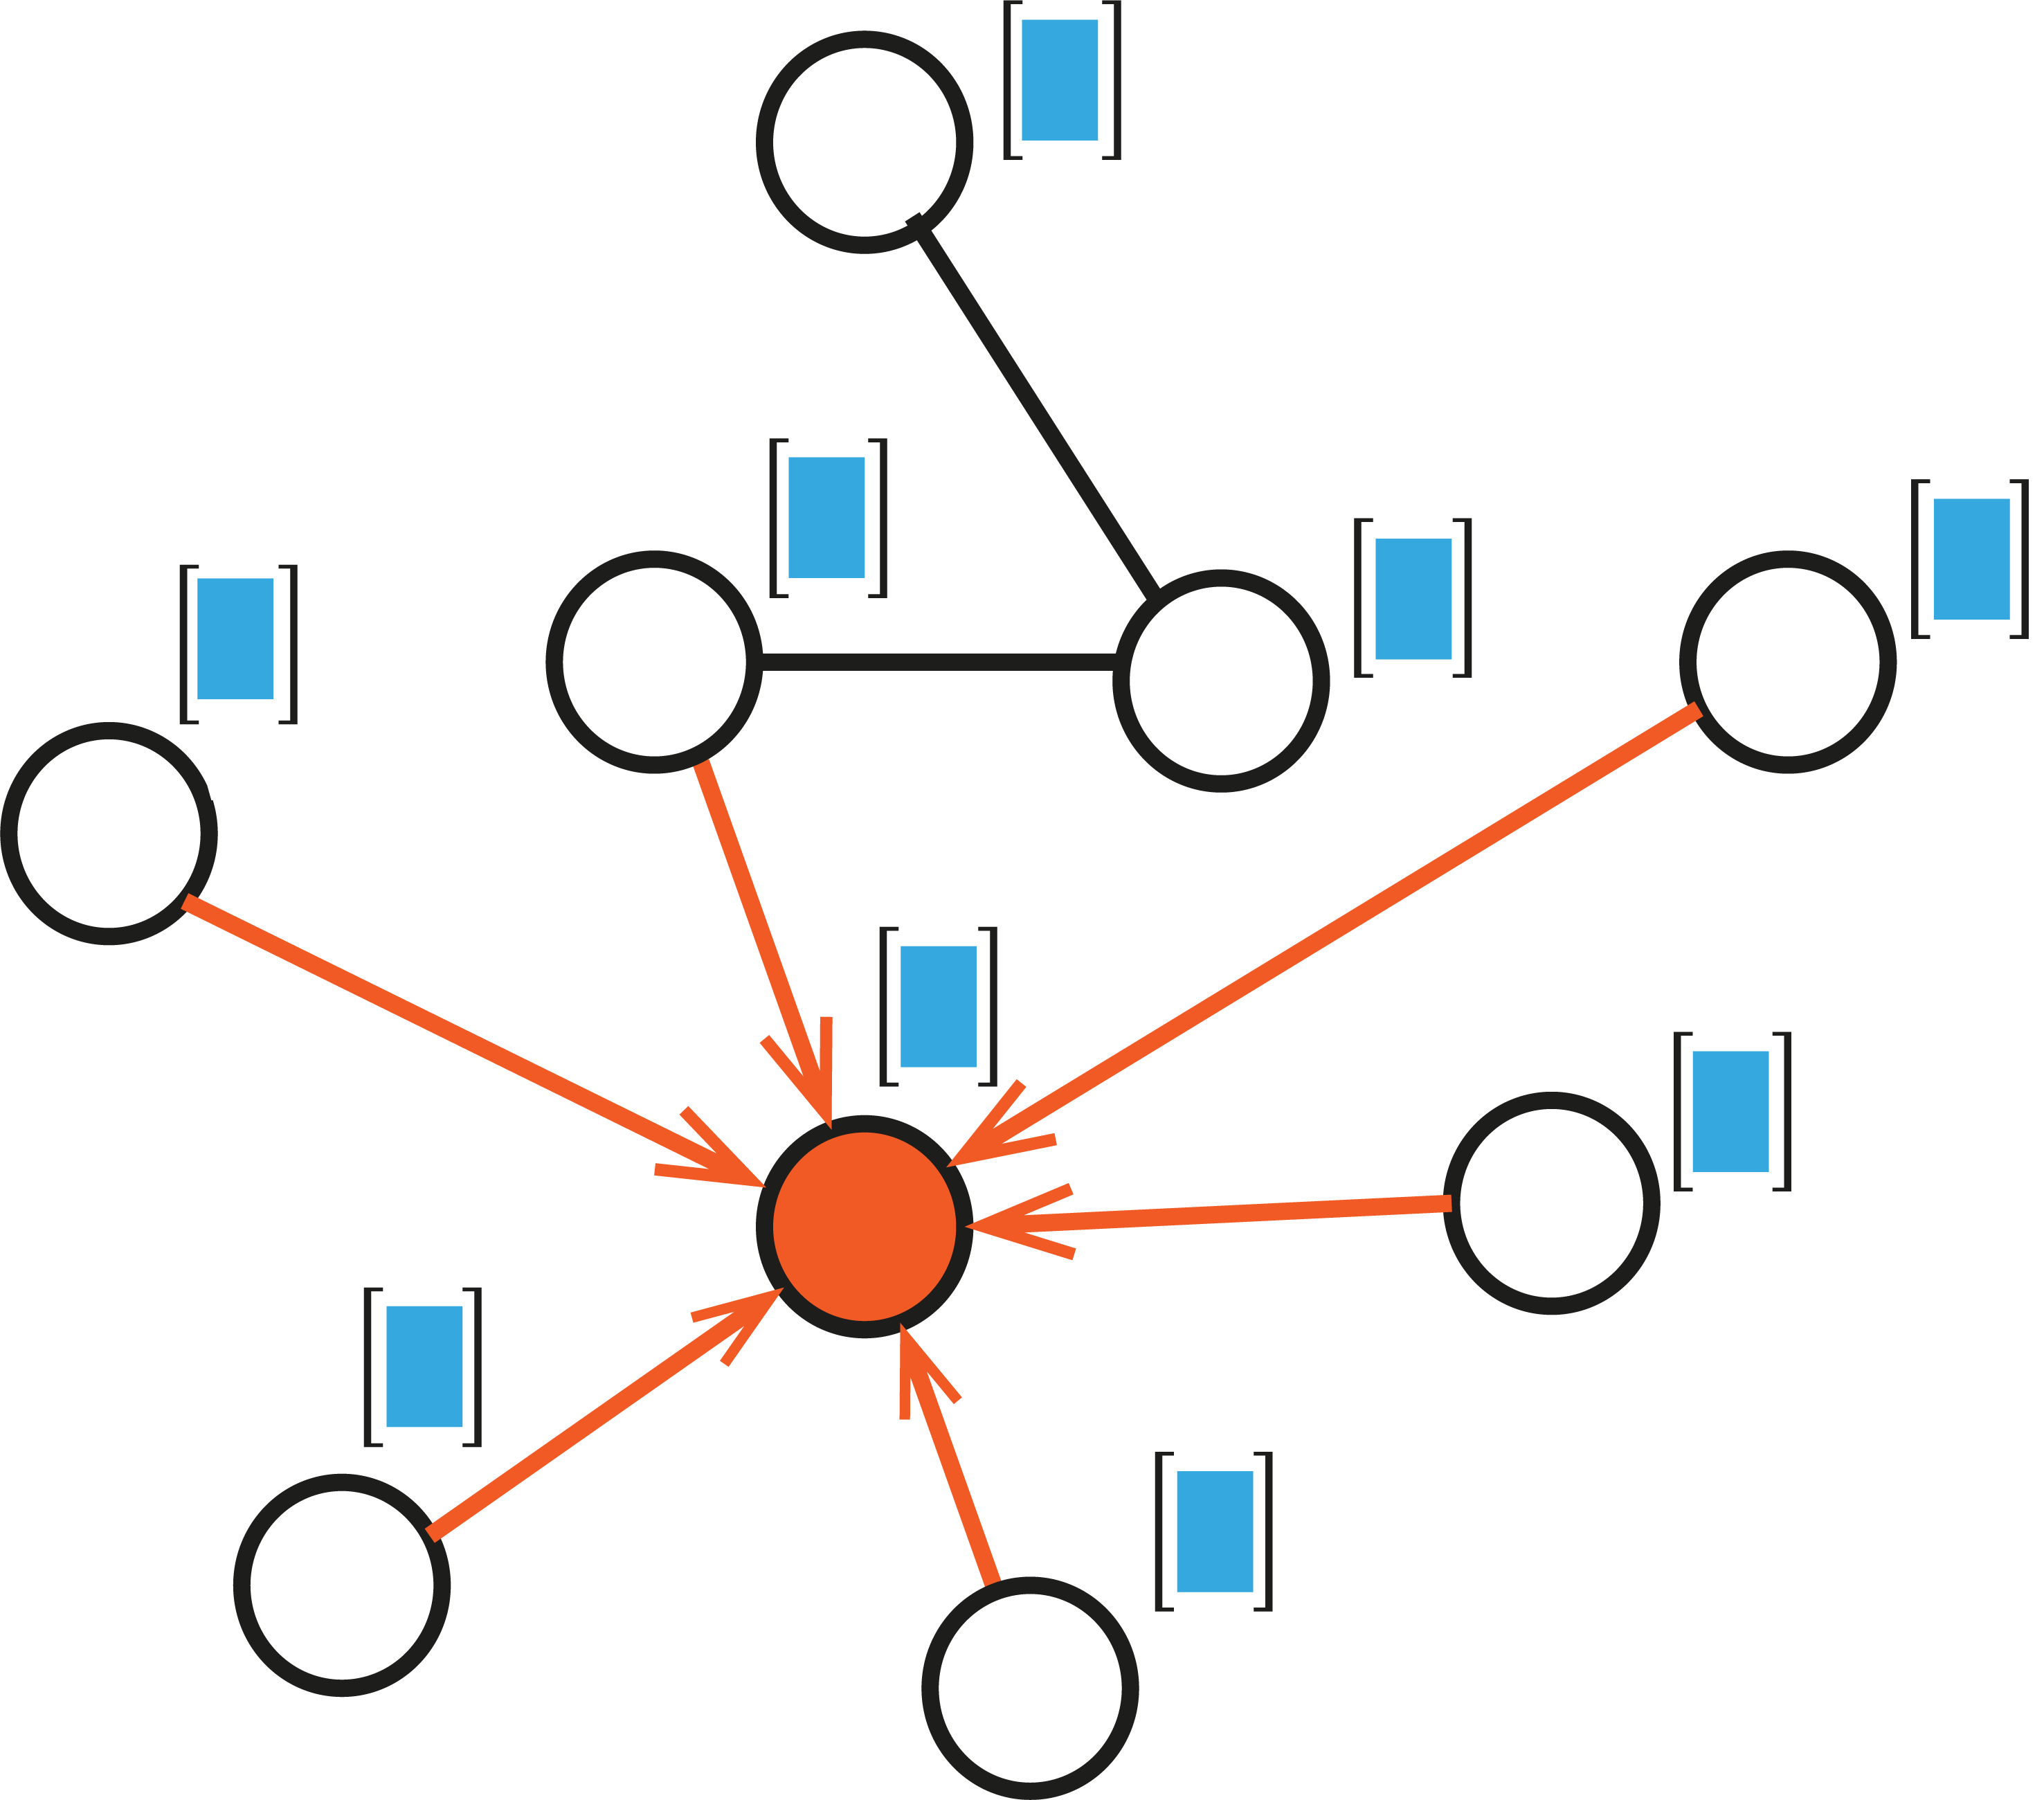
\includegraphics[scale=.20]{figures/introduction/deepspeed-gnns.png}
                    \caption*{\scriptsize Message Aggregation in Graph Convolutional Neural Networks}
                \end{figure}
                \vspace*{-1cm}
                \begin{figure}[H]
                    \centering
                    \captionsetup{justification=centering}
                    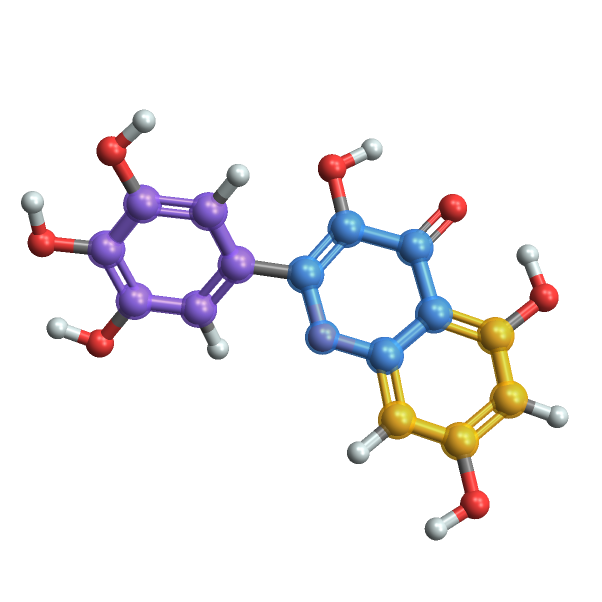
\includegraphics[scale=.15]{figures/introduction/molecular_graph.png}
                    \vspace{-0.25cm}
                    \caption*{\scriptsize Molecule represented as Graph structure\footnotemark}
                \end{figure}
            \end{center}
        \end{column}
    \end{columns}
    \footnotetext{\url{https://www.wolfram.com/}}
\end{frame}
